\section{Introduction}

\textit{Wireless sensor networks (WSNs)} have many environmental monitoring applications and on-going research in areas such as oceanographic measurement \citep{Mahdy2008a, Albaladejo2010, 6973877}, radioactive contamination \citep{Gomez2015}, water quality \citep{Fang2010}, flood levels \citep{Castillo2004}, volcanic activity \citep{Werner-Allen2006}, agricultural soil \citep{8745854}, as well as in military uses \citep{6268958}. More recently, the availability and lower cost of low-power wireless transmitters \citep{902661}, solar-harvesting components \citep{Prauzek2018}, and micro-electro-mechanical systems \citep{1045391} has allowed large deployment sizes and increased the scope of use, expanding their real-world applications and opening up new areas for research \citep{5597912, Kandris2020}.

WSNs can be structured with centralised or decentralised control. With centralisation, the controller node has system-wide knowledge, and so allocates measurement tasks to other nodes, orchestrates their communications, and handles recovery (see Figure \ref{fig:wsn_centralised}). This approach does not scale well to large networks due to congestion and resource exhaustion on the central component. In harsh environments, this centralisation of control is not robust to damage or node loss. Although some adaptivity can be added to these systems to help them optimise in complex systems, non-distributed learning algorithms suffer from the same limitations as non-learning WSN systems \citep{Imagestate2006}. For these reasons, we focus on decentralised, autonomous methods.

With decentralised WSNs, nodes have limited knowledge of the system. Each node acts autonomously to some degree to orchestrate the functionality mentioned above. They are often organised into groups to decrease the cost of coordination without full centralisation. The basis of many of these decentralised techniques is hierarchical, typically some form of clustering technique. Nodes are formed into sub-groups with designated leaders that orchestrate the behaviours of each group of nodes and communicates with the central controller (see Figure \ref{fig:wsn_clustering}) . This ability for nodes to work autonomously increases resilience but introduces new challenges. In working with local information only, the system can fail to optimise well or get trapped in local optima. In addition, system-wide coordination of node behaviours is difficult when communication is limited to small sets of neighbours \citep{Carlos-Mancilla2016}. Reinforcement learning has seen applications in these decentralised systems, often focussed on using adaptive routing  to optimise energy efficiency and system lifetime \citep{ 10.1504/IJCNDS.2012.048871, Kulkarnib}, or to ensure sensor coverage is maintained with the loss of nodes over time \citep{Sharma2020}. These solutions look at single or complementary objective optimisation, and do not take account of the conflicting multiple objectives in WSN systems. System goals may involve energy optimisation, coverage, measurement quality, and how nodes allocate resources to meet these goals. 

\begin{figure}
	\begin{subfigure}{0.5\textwidth}
		\centering
		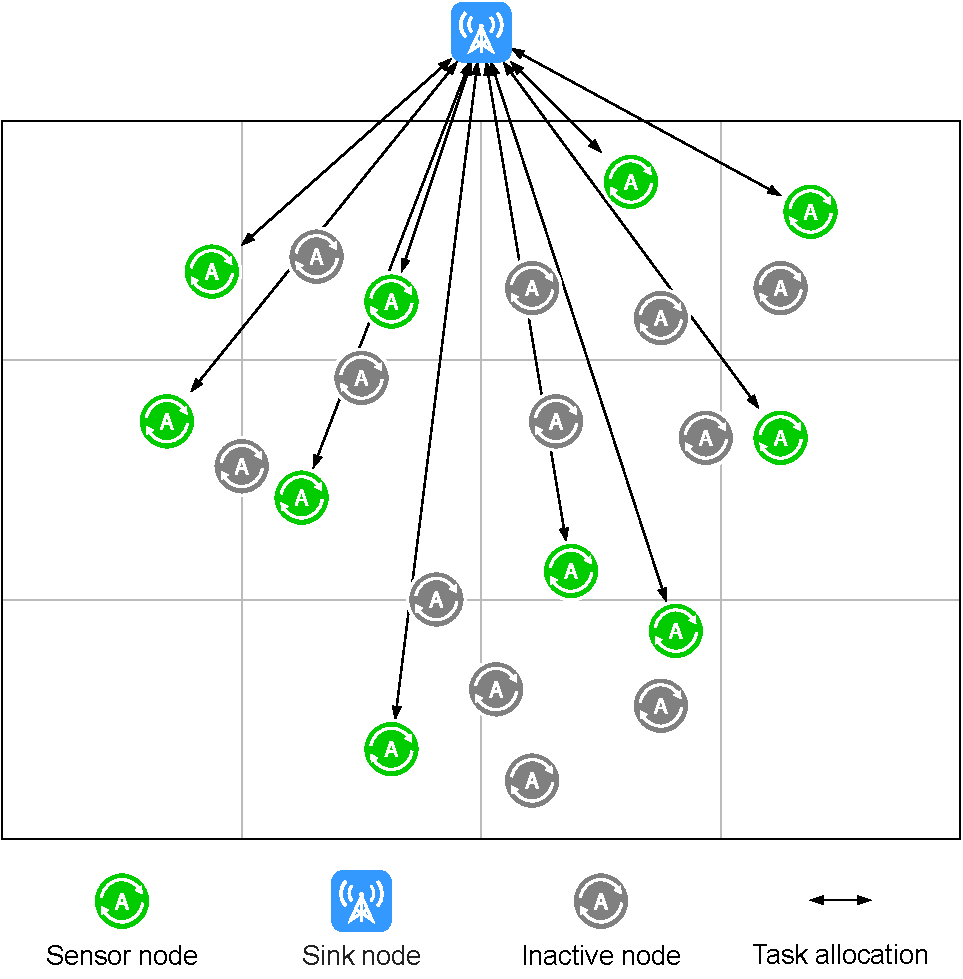
\includegraphics[width=.8\linewidth]{WSN_centralised}
		\caption{A centralised WSN configuration with direct communication}
		\label{fig:wsn_centralised}
	\end{subfigure}%
	\begin{subfigure}{0.5\textwidth}
		\centering
		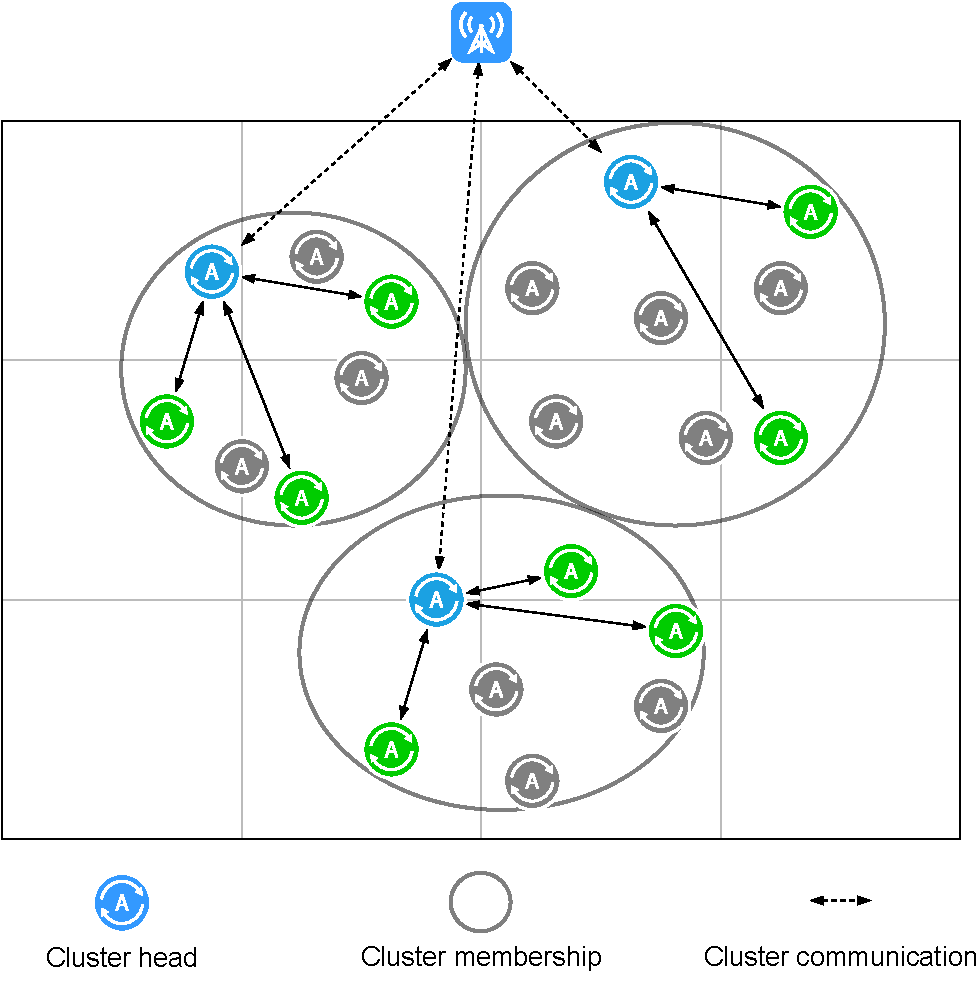
\includegraphics[width=.8\linewidth]{WSN_clustering}
		\caption{A decentralised WSN configuration based on clustering}
		\label{fig:wsn_clustering}
	\end{subfigure}
	\caption{Common WSN configurations for task coverage of a grid}
	\label{fig:wsn_centralised_decentralised}
\end{figure}

As a solution to the challenge of optimising for multiple, competing objectives in a WSN system, we present the \acronymWSNOptimisationExtended{}{} algorithm. Using a reinforcement learning approach, it adapts the probabilities of agents taking different actions by learning from the outcome of past task completions. In doing so, it alters agents' behaviour to optimise for overall energy efficiency in the system, and the quality of task completions. The algorithm can be shown to improve the sensor coverage, the network resilience of the WSN, and to increase the systems' useful lifetime. Additionally the algorithm adapts the allocation of agents' resources needed to complete tasks to improve the quality of their completion, increasing the system utility.  We evaluated the performance of the  algorithm in a number of simulation types of a realistic environmental monitoring scenario. This work builds on the  \acronymATARIA{}{} and \acronymMGRAO{}{} algorithms previously developed by the authors  \citep{creech2021dynamic, creech2021resource}. 

The structure of the paper is as follows. In Section \ref{section:background} we look at related research in this area, allowing us to concretely define the problem in Section \ref{section:problem}. Section \ref{section:solution} sets out our solution, followed by definition of the simulated environment and evaluation of the solution in Section \ref{section:experimental}. We close with the summary of our conclusions and future work in Section \ref{section:conclusions}.
